Esse capítulo apresenta os resultados obtidos com o desenvolvimento do sistema web, e com as consultas feitas tanto para obter informações relevantes sobre a CEAP, quanto para detectar possíveis fraudes.

\section{Consultas CEAP - TSE}

O sistema web recebeu o nome de "CEAP Colaborativo". Na tela inicial são apresentados algumas informações importantes para a compreensão do objetivo do sistema. A tela inicial pode ser vista na Figura \ref{fig:sistema_ceap}

\begin{figure}[H]
\centering
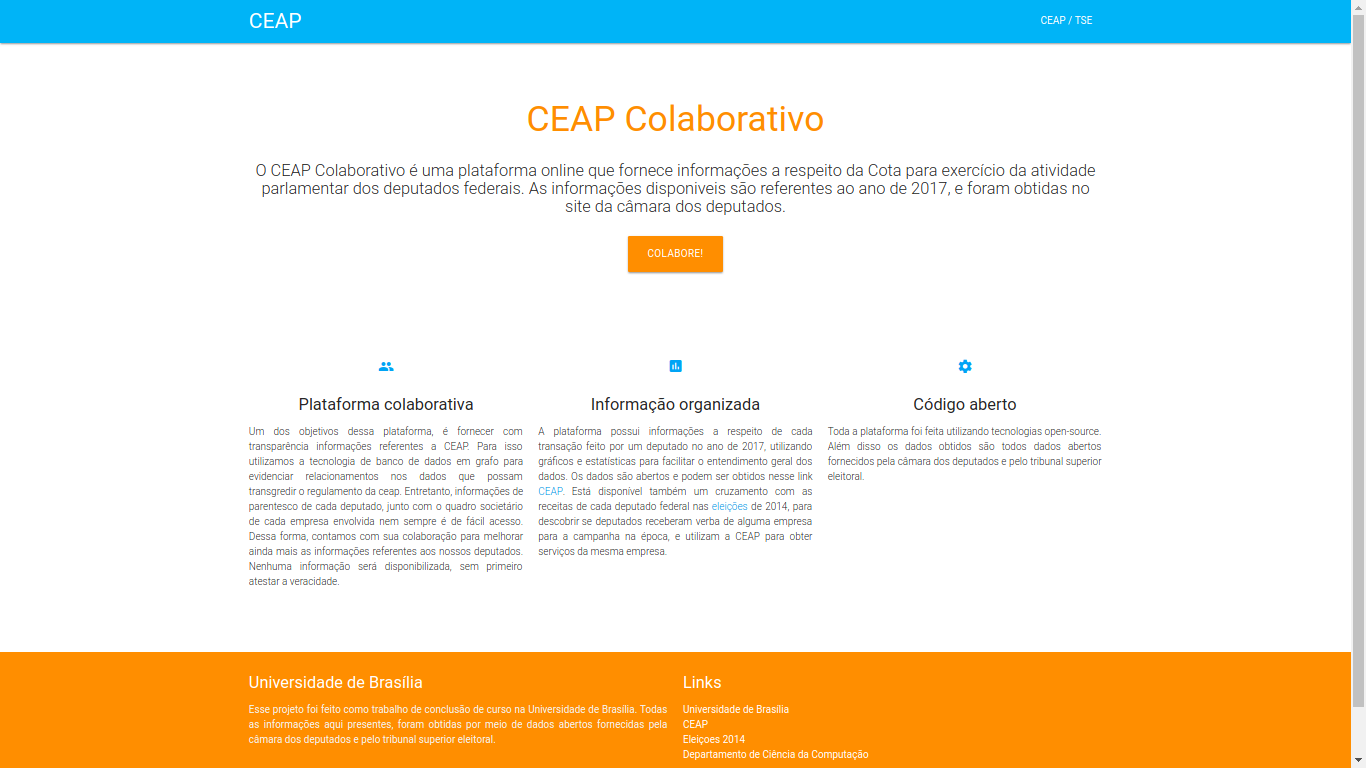
\includegraphics[width=.75\textwidth]{sistema_ceap.png}
\caption{Tela inicial do sistema "CEAP Colaborativo"}
\label{fig:sistema_ceap}
\end{figure}

A partir desta tela inicial, é possível navegar para as demais telas utilizando a barra azul de navegação. Nessa barra de navegação ao clicar no link "CEAP / TSE" o sistema redireciona o usuário para uma tela que fornece informações gerais a respeito do conjunto de dados utilizado. A figura \ref{fig:sistema_ceap_tse} mostra a parte inicial da tela "CEAP / TSE":

\begin{figure}[H]
\centering
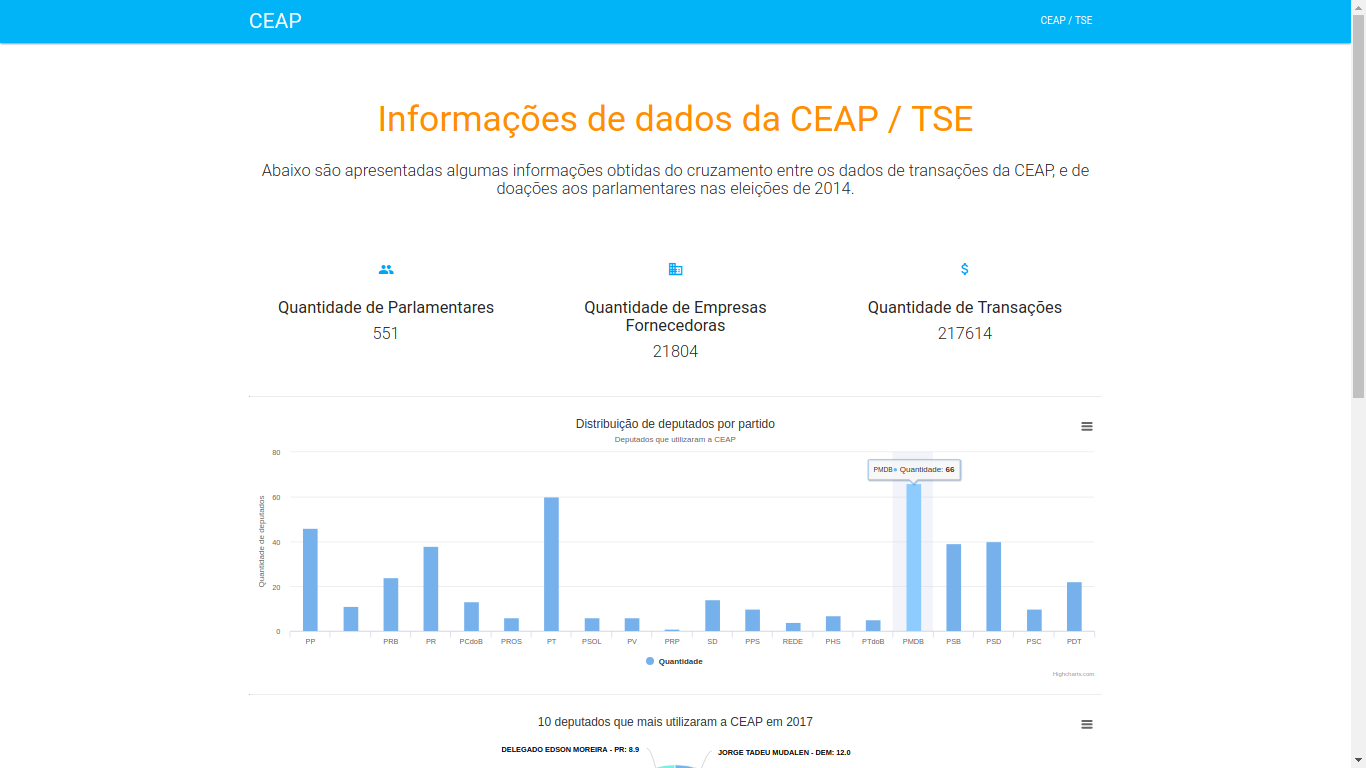
\includegraphics[width=.75\textwidth]{ceap-tse.png}
\caption{Tela de informações gerais do sistema "CEAP Colaborativo"}
\label{fig:sistema_ceap_tse}
\end{figure}

No início da tela é informado que foram armazenados no banco de dados um total de 551 parlamentares, 21804 empresas fornecedoras e 217614 transações.
A primeira consulta feita nesta tela foi a distribuição de deputados que utilizaram a CEAP por partido. A Figura \ref{fig:chart_1} apresenta o resultado.

\begin{figure}[H]
\centering
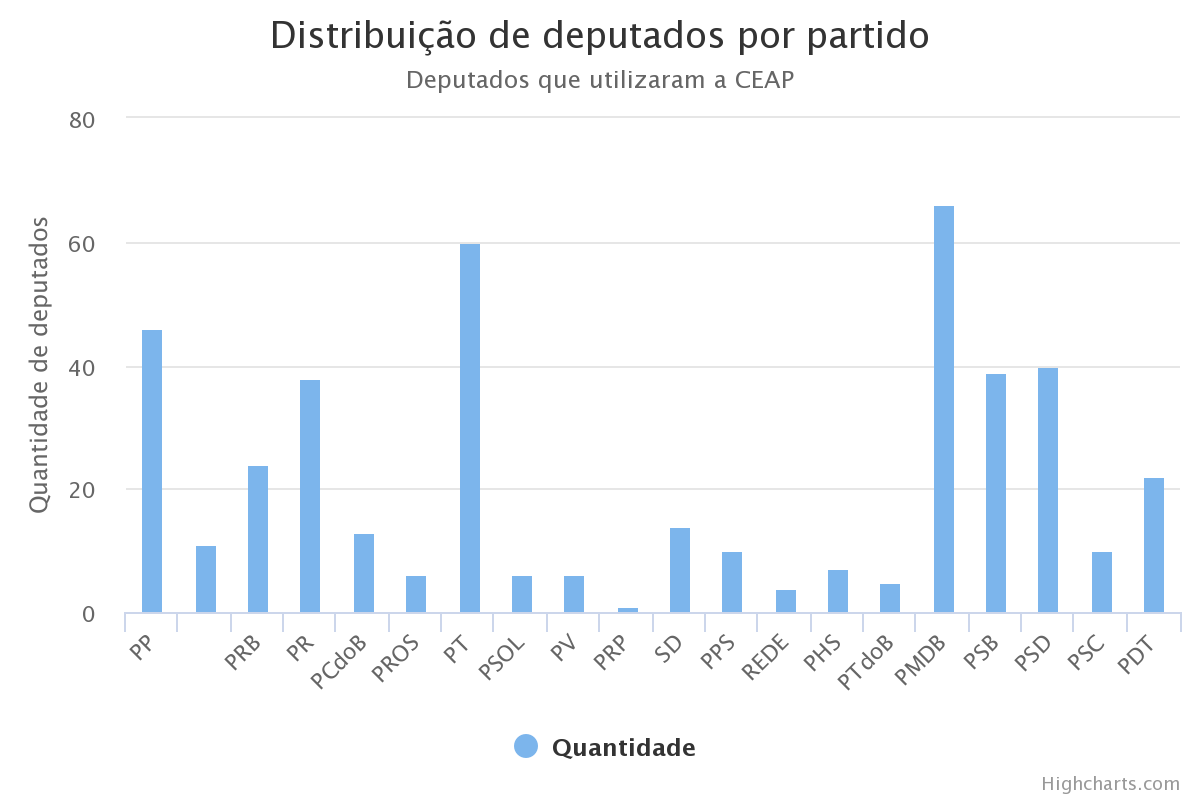
\includegraphics[width=.75\textwidth]{chart_1.png}
\caption{Distribuição de deputados que utilizaram a CEAP por partido}
\label{fig:chart_1}
\end{figure}

\begin{lstlisting}[label={lst:consulta_chart_1}, caption={Consulta para o gráfico \ref{fig:chart_1}},captionpos=b, language=sql]
select SgPartido, count(SgPartido) from Parlamentar GROUP BY SgPartido
\end{lstlisting}

A partir do gráfico \ref{fig:chart_1} é possível observar que o partido que tem mais deputados que utilizaram a CEAP no ano de 2017 foi o PMDB com 66 deputados, seguido pelo PT com 60 deputados, e pelo PP com 46 deputados. É interessante notar como o OrientDB mesmo sendo um SGBD NoSQL, possui uma linguagem baseada na linguagem de consulta SQL e portanto a consulta \ref{lst:consulta_chart_1} se assemelha bastante a uma consulta SQL de um SGBD relacional.

A próxima consulta feita foi para obter os 10 deputados que mais fizeram transações no ano de 2017. A figura \ref{fig:chart_2} apresenta o resultado.

\begin{figure}[H]
\centering
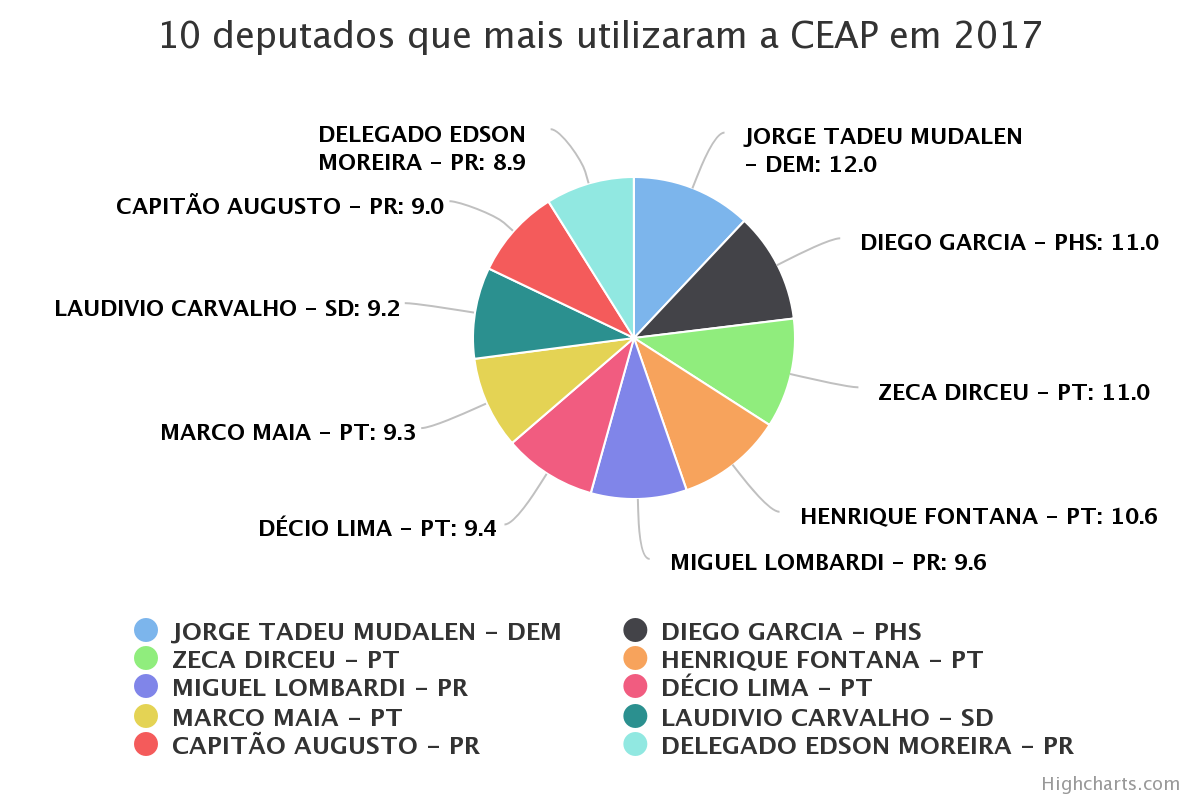
\includegraphics[width=.75\textwidth]{chart_2.png}
\caption{10 deputados que mais fizeram transações no ano de 2017}
\label{fig:chart_2}
\end{figure}

\begin{lstlisting}[label={lst:consulta_chart_2}, caption={Consulta para o gráfico \ref{fig:chart_2}},captionpos=b, language=sql]
select TxNomeParlamentar, SgPartido, out("RealizaTransacao").size() 
as transacoes from Parlamentar 
order by transacoes desc limit 10
\end{lstlisting}

Por meio do gráfico \ref{fig:chart_2}, percebe-se que o deputado que mais realizou transações foi o Jorge Tadeu Mudalen do partido DEM com 1280 transações, seguido pelo Diego Garcia do PHS com 1176 transações, e pelo Zeca Dirceu do PT com 1173 transações. A consulta \ref{lst:consulta_chart_2} por sua vez, possui elementos específicos do OrientDB, que no caso é a função "out". Nessa consulta são selecionados o nome do parlamentar, o partido do parlamentar e a quantidade de arestas de classe "RealizaTransacao" saindo do parlamentar. Essa consulta é ordenada de forma decrescente pela quantidade de arestas que saem de um parlamentar, e limitada para obter os 10 primeiros.

A próxima consulta feita foi feita para obter as 15 empresas fornecedoras que mais forneceram serviços aos deputados em 2017. A figura \ref{fig:chart_3} apresenta o resultado.

\begin{figure}[H]
\centering
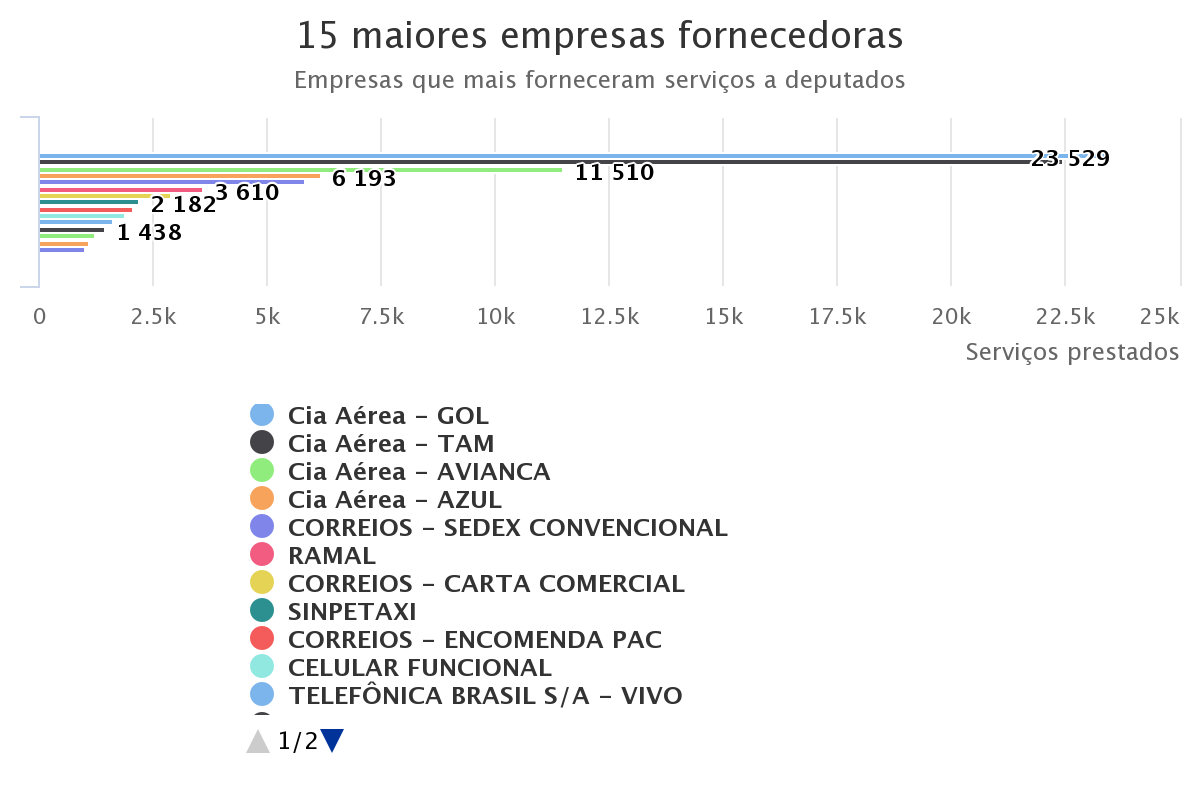
\includegraphics[width=.75\textwidth]{chart_3.png}
\caption{15 empresas fornecedoras que mais forneceram serviços aos deputados em 2017}
\label{fig:chart_3}
\end{figure}

\begin{lstlisting}[label={lst:consulta_chart_3}, caption={Consulta para o gráfico \ref{fig:chart_3}},captionpos=b, language=sql]
select TxtFornecedor, in("FornecidaPor").size() as servicos 
from EmpresaFornecedora 
order by servicos desc limit 15
\end{lstlisting}

A partir do gráfico \ref{fig:chart_3}, percebe-se que as quatro primeiras empresas que mais forneceram serviços com a verba da CEAP são do ramo de aviação. Um dos propósitos da CEAP é justamente para a compra de passagens de avião, principalmente entre deputados de outros estados que não sejam o Distrito Federal. A Cia Aérea GOL lidera essa estatística com um total de 23529 transações. A consulta \ref{lst:consulta_chart_3} também possui elementos específicos do OrientDB, agora no caso a função "in". Nessa consulta são selecionados da classe "EmpresaFornecedora", o nome do fornecedor e a quantidade de arestas de classe "FornecidaPor" que entram no vértice. Em seguida é ordenada de forma decrescente pela quantidade de arestas mencionada e limitada para obter as 15 primeiras empresas.

Finalmente a última consulta busca identificar no formato de um grafo parlamentares que usaram a CEAP com empresas que fizeram doações para a campanha desse parlamentar em 2014. Esse resultado foi mostrado no formato de grafo na Figura \ref{fig:ceap_tse_graph}, mas esse resultado utiliza a ferramenta gráfica presente no OrientDB. Nesse caso a consulta foi feita e a partir do \textit{JSON} obtido foi construído um grafo na camada de apresentação do sistema desenvolvido. A Figura \ref{fig:sigma} apresenta o resultado.

\begin{figure}[H]
\centering
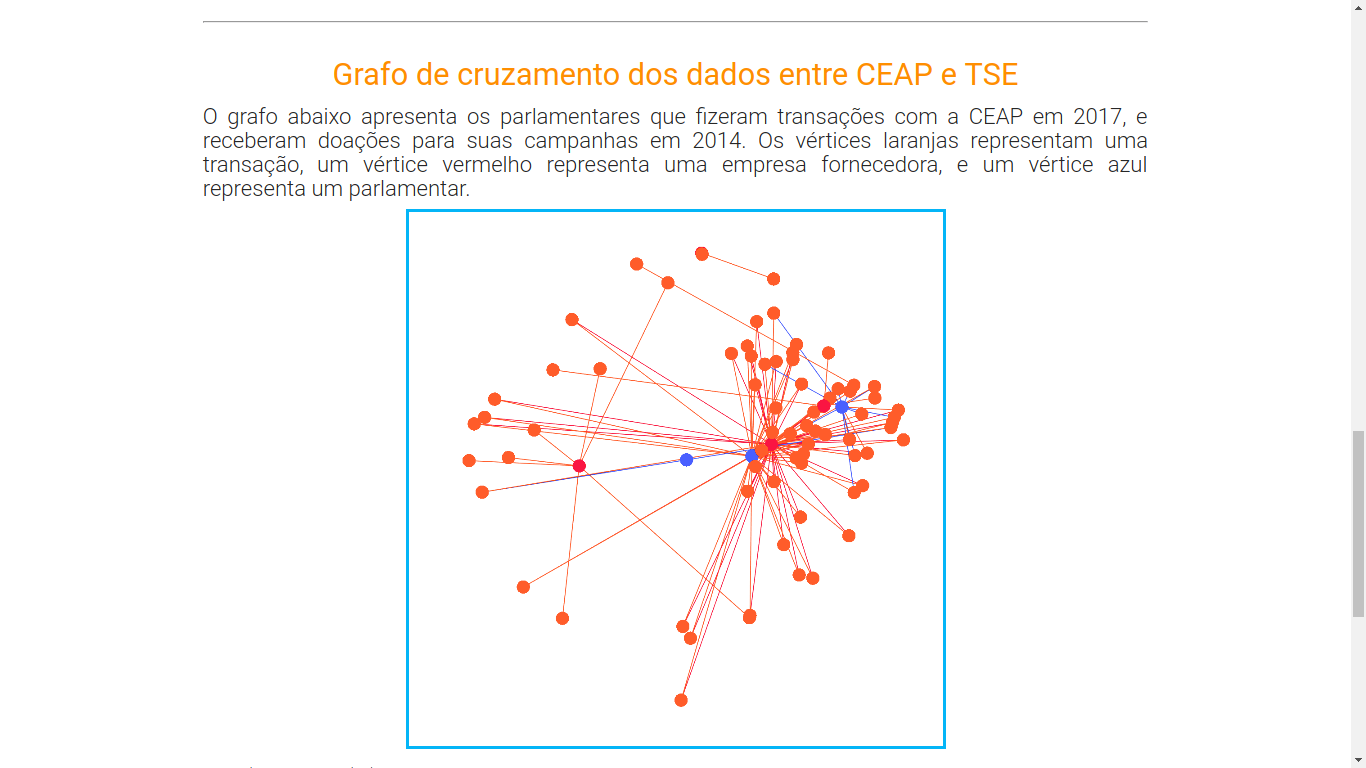
\includegraphics[width=.75\textwidth]{sigma.png}
\caption{Grafo na camada de apresentação com dados do cruzamento entre as bases da CEAP e do TSE.}
\label{fig:sigma}
\end{figure}

O gráfico utilizado na camada de apresentação possui algumas limitações, e não é robusto como o grafo apresentado pelo OrientDB. De ambas as formas foi possível encontrar o seguinte relacionamento entre deputados e empresas fornecedoras.

\begin{table}[h!]
\centering
\begin{tabular}{|l|l|l|l|l|}
\hline
Deputado & Empresa Fornecedora \\ \hline
AELTON FREITAS & Auto Posto Cortez Ltda \\ \hline
DIEGO ANDRADE & Grafica Mundial LTDA-ME \\ \hline
MARCELO ARO & SEMPRE EDITORA LTDA. \\ \hline
WELITON PRADO & SEMPRE EDITORA LTDA. \\ \hline
TONINHO PINHEIRO & SEMPRE EDITORA LTDA. \\ \hline
MARCUS PESTANA & SOLAR COMUNICAÇÕES S.A \\ \hline
EROS BIONDINI & TARGET RENT A CAR LTDA \\ \hline
\end{tabular}
\caption{Relacionamento entre deputados e empresas fornecedoras}
\label{table:relation_deputies_companies}
\end{table}

\section{Consultas CEAP para detectar fraudes}

O "CEAP Colaborativo" tem com um dos objetivos permitir que a população contribua com informações que podem ajudar na detecção de fraudes da CEAP. Tais informações podem ser em relação a parentes dos deputados e quadros de sócios das empresas fornecedoras. Portanto ao clicar no link "Contribuir" na barra de navegação, o usuário é redirecionado para uma tela com formulários que permitem que as informações sejam submetidas. A Figura abaixo apresenta a tela em questão.

imagem....

Ao fornecer os dados, não é feita a persistência imediatamente. Usuários administradores precisam analisar se a informação fornecida é verídica. Após essa verificação, o dado pode ser aceito ou rejeitado.

Ao clicar no link fraudes, o sistema redireciona o usuário para uma tela que contém consultas com o objetivo de encontrar padrões que violam as regras da CEAP. Para fins de validação, foram utilizados dados fictícios para testar as consultas realizadas. A primeira análise apresentada, refere-se a consulta \ref{fig:socios} que consegue localizar um padrão de transações efetuadas entre um deputado e uma empresa, na qual o deputado faz parte do quadro de sócios. A figura abaixo apresenta os resultados.

imagem....

Por fim foi feita uma consulta que busca transações feitas com a CEAP para empresas na qual parentes do deputado fazem parte do quadro societário.A figura abaixo apresenta os resultados.

imagem....